\documentclass[a4paper, 12pt]{article}%тип документа



%отступы
\usepackage[left=1cm,right=1cm,top=1cm,bottom=2cm,bindingoffset=0cm]{geometry}

%%% Работа с русским языком
\usepackage{graphicx}
\usepackage{cmap}                           % поиск в PDF
\usepackage{mathtext} 			 	       % русские буквы в формулах
\usepackage[T2A]{fontenc}               % кодировка
\usepackage[utf8]{inputenc}              % кодировка исходного текста
\usepackage[english,russian]{babel} 
\usepackage{float}

\usepackage[export]{adjustbox} % локализация и переносы

\usepackage{subfig}% http://ctan.org/pkg/subfig
\usepackage{booktabs}

\usepackage{wrapfig}


%Матеша
\usepackage{amsmath,amsfonts,amssymb,amsthm,mathtools} % AMS
\usepackage{icomma} % "Умная" запятая

%\mathtoolsset{showonlyrefs=true} % Показывать номера только у тех формул, на которые есть \eqref{} в тексте.

%% Шрифты
\usepackage{euscript}	 % Шрифт Евклид
\usepackage{mathrsfs} % Красивый матшрифт

%% Свои команды
\DeclareMathOperator{\sgn}{\mathop{sgn}}

%% Перенос знаков в формулах (по Львовскому)
\newcommand*{\hm}[1]{#1\nobreak\discretionary{}
	{\hbox{$\mathsurround=0pt #1$}}{}}


\date{27.09.2022}

\author{Гаврилин Илья Дмитриевич \\
	Б01-101}
\title{\textbf{Работа 3.3.2 \\ 
		Исследование вольт-амперной характеристики вакуумного диода}}


\begin{document}
	\maketitle
	\section{Аннотация}
	В работе рассчитывается удельный заряд электрона (заряд на единицу массы: $e/m$). Для его определения применяется закон "трех вторых": $I = A_0 U^{3/2}$. В качестве элемента, на котором выполняется данный закон используется вакуумная лампа, для которой измеряется зависимость анодного напряжения от анодного тока, при различных значениях тока накала.
	\section{Теоретические сведения}
	В работе исследуется зависимости прямого тока, проходящего через вакуумный диод, в зависимости от напряжения на нем, а именно та часть вольт-амперной характеристики, в которой электронное облако существенно влияет на распределение электрического поля между катодом и анодом.
	
	Распределение потенциала по радиусу внутри диода определяется уравнением Пуассона в цилиндрических координатах:
	
	\begin{equation}\label{}
		\Delta V = \dfrac{d^2V}{dr^2} + \dfrac{1}{r} + \dfrac{dV}{dr} = - \dfrac{\rho(r)}{\epsilon_0}
	\end{equation}
	
	При этом плотность заряда $ \rho(r) $ связана с текущим через слой диода толщины $ l $ током $ I $ формулой $ I = -2\pi r \rho(r)v(r)l$. При этом из закона сохранения энергии мы легко находим скорость $ v(r) $ электронов , прошедших через разность потенциалов $ V(r) $: $ \frac{mv^2}{2} = eV(r) $.  Отсюда мы получаем уравнение 
	
	\begin{equation}\label{ur}
		r \dfrac{d^2V}{dr^2} + \dfrac{dV}{dr} = \dfrac{I}{2\pi\epsilon_0}\sqrt{\dfrac{m}{2eV}}
	\end{equation}
	
	Однако, в дифференциальном уравнении 2-ого порядка относительно $ V(r) $ нам неизвестен ток I, зависящий от V. Для доопределения уравнения будем полагать:
	
	\begin{equation}\label{usl}
		\dfrac{dV}{dt}\bigg |_{r=r_k} = 0
	\end{equation} 
	
	Наше предположение означает что вблизи катода пространственный заряд электронов полностью экранирует поле анодной разности потенциалов.
	
	Уравнение \eqref{ur} является нелинейным. Попробуем  найти некое частное решение, где $ V_a = V_{a0}, $ при котором ток $ I = I_0 $. Тогда выражения 
	
	\begin{equation}\label{}
		I = I_o \left( \dfrac{V_a}{V{a0}} \right) ^{3/2}, \qquad V(r) = V_{a0}(r)\dfrac{V_a}{V_{a0}}
	\end{equation}
	
	являются решением уравнения \eqref{ur}, что проверяется подстановкой. В общем виде решение записывается в виде
	
	\begin{equation}\label{3/2}
		I = \dfrac{8\sqrt{2}\pi \epsilon_0 l}{9}\sqrt{\dfrac{e}{m}}\dfrac{1}{r_a\beta^2} V^{3/2}
	\end{equation}
	
	Это и есть так называемый "<закон трех вторых"> -- ток в вакуумном диоде пропорционален напряжению на нем в степени 3/2. Он справедлив при любой геометрии электродов, если ток не слишком велик (т.е. пока выполнено условие \eqref{usl}). 
	
	Так как нам нужно найти удельный заряд электрона, выпишем в явном виде его из уравнения \eqref{3/2}:
	
	\begin{equation}\label{e/m}
		\dfrac{e}{m} = \dfrac{81r_a^2\beta^4}{128\pi^2\epsilon_0^2l^2}  \dfrac{I^2}{V^2} = k  \dfrac{I^2}{V^3} = k (\frac{dI}{dV^{3/2}})^2
	\end{equation}
	
	Таким образом, удельный заряд электрона определяется из отношения квадрата тока к кубу напряжения, умноженный на коэффициент, зависящий от параметров установки.
	\section{Ход работы}
	\subsection{Рассчет k}
	В работе используется диод 2Ц2С с косвенным накалом. Радиус его катода $ r_k = 0,9 $ мм, радиус анода $ r_a = 9,5  $ мм, коэффициент $ \beta^2 = 0,98 $, длина слоя центральной части катода, покрытой оксидным слоем $ l = 9 $ мм.
	
	Для подогрева катода и анода используются стабилизированные источники постоянного тока и напряжения. В цепь накала включено предохранительное напряжение $ R $. Анодное напряжение измеряется вольтметром источника питания, анодный ток --- многопредельным мультиметром GDM-8245. 
	
	\begin{figure}[H]
		\centering
		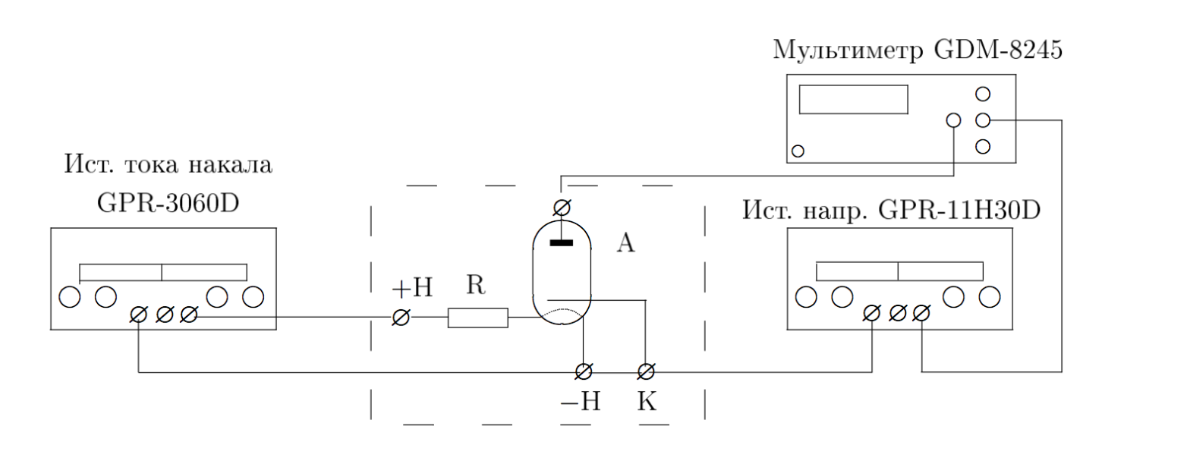
\includegraphics[width=0.8\linewidth]{scheme}
		\caption{Схема экспериментальной установки}
		\label{fig:scheme}
	\end{figure}
	Вычислим коэффициент $ k $:
	
	\begin{equation}\label{}
		k = \dfrac{81r_a^2\beta^4}{128\pi^2\epsilon_0^2l^2} = \dfrac {81\cdot(9,5\cdot10^{-3})^2\cdot0,98^4}{64\cdot2\cdot3,14^2\cdot(8,85\cdot10^{-12})^2\cdot(9\cdot10^{-3})^2} \approx 8,4 \cdot 10^{20}
	\end{equation}
	\subsection{Замеры}
	Проведем замеры анодной ВАХ для диода, на 4-ех различных значениях накального тока: 1.3, 1.4, 1.5, 1.6 А.
	\begin{table}[H]
		\centering
		\begin{tabular}{|c|c|c|c|c|}
			\hline
			$I_H$, A & 1.3     & 1.4     & 1.5     & 1.6     \\ \hline
			$U_а$, В    & $I_а,~ \mu A$   & $I_а,~ \mu A$   & $I_а,~ \mu A$   & $I_а,~ \mu A$   \\ \hline
			0.5     & 4.19    & 8.21    & 15.76   & 22.97   \\ \hline
			1.0     & 12.56   & 19.68   & 27.46   & 40.85   \\ \hline
			1.5     & 24.50   & 32.75   & 44.71   & 58.90   \\ \hline
			2.0     & 40.84   & 48.38   & 62.94   & 77.85   \\ \hline
			2.5     & 56.10   & 66.74   & 82.44   & 101.50  \\ \hline
			3.0     & 74.21   & 86.33   & 104.42  & 122.59  \\ \hline
			3.5     & 93.26   & 110.53  & 126.56  & 146.34  \\ \hline
			4.0     & 115.00  & 130.04  & 149.13  & 171.78  \\ \hline
			4.5     & 138.76  & 157.73  & 175.74  & 197.36  \\ \hline
			5.0     & 160.84  & 179.68  & 203.47  & 229.12  \\ \hline
			5.5     & 188.38  & 206.56  & 231.02  & 255.30  \\ \hline
			6.0     & 211.97  & 231.84  & 255.75  & 285.96  \\ \hline
			7.0     & 268.20  & 291.45  & 321.18  & 352.82  \\ \hline
			8.0     & 330.72  & 357.62  & 386.84  & 423.84  \\ \hline
			9.0     & 397.92  & 428.73  & 458.31  & 496.30  \\ \hline
			10.0    & 494.00  & 496.77  & 570.50  & 609.50  \\ \hline
			15.0    & 906.40  & 954.00  & 1002 & 1062 \\ \hline
			20.0    & 1417 & 1476 & 1545 & 1609 \\ \hline
			25.0    & 2005 & 2090 & 2165 & 2235 \\ \hline
			30.0    & 2642 & 2753 & 2838 & 2930 \\ \hline
			35.0    & 3323 & 3470 & 3565 & 3654 \\ \hline
			40.0    & 4036 & 4226 & 4345 & 4444 \\ \hline
			45.0    & 4781 & 5046 & 5243 & 5365 \\ \hline
			50.0    & 5646 & 6000 & 6141 & 6270 \\ \hline
		\end{tabular}
		\caption{Замеры ВАХ вакуумного диода}
	\end{table}
	\subsection{Построение графиков}
	Построим зависимость $I=f(U^{3/2})$, из коэффициента наклона определим значение производной: $\frac{dI}{dV^{3/2}}$.\\
	При построении графика учтем что ВАХ может в некоторых местах не совпадать с законом <<трех вторых>> , поэтому при аппроксимации прямой в качестве данных будем брать точки начиная с некоторой (4-5 точка для всех графиков), для меньших значений анодного напряжения понижается точность замера тока мультиметром. \\
	По линейности графика на большинстве замеров можем сделать выводы о справедливости закона, продолжим расчеты удельного заряда электрона, используя полученные данные.
	\begin{figure}[H]
		\centering
		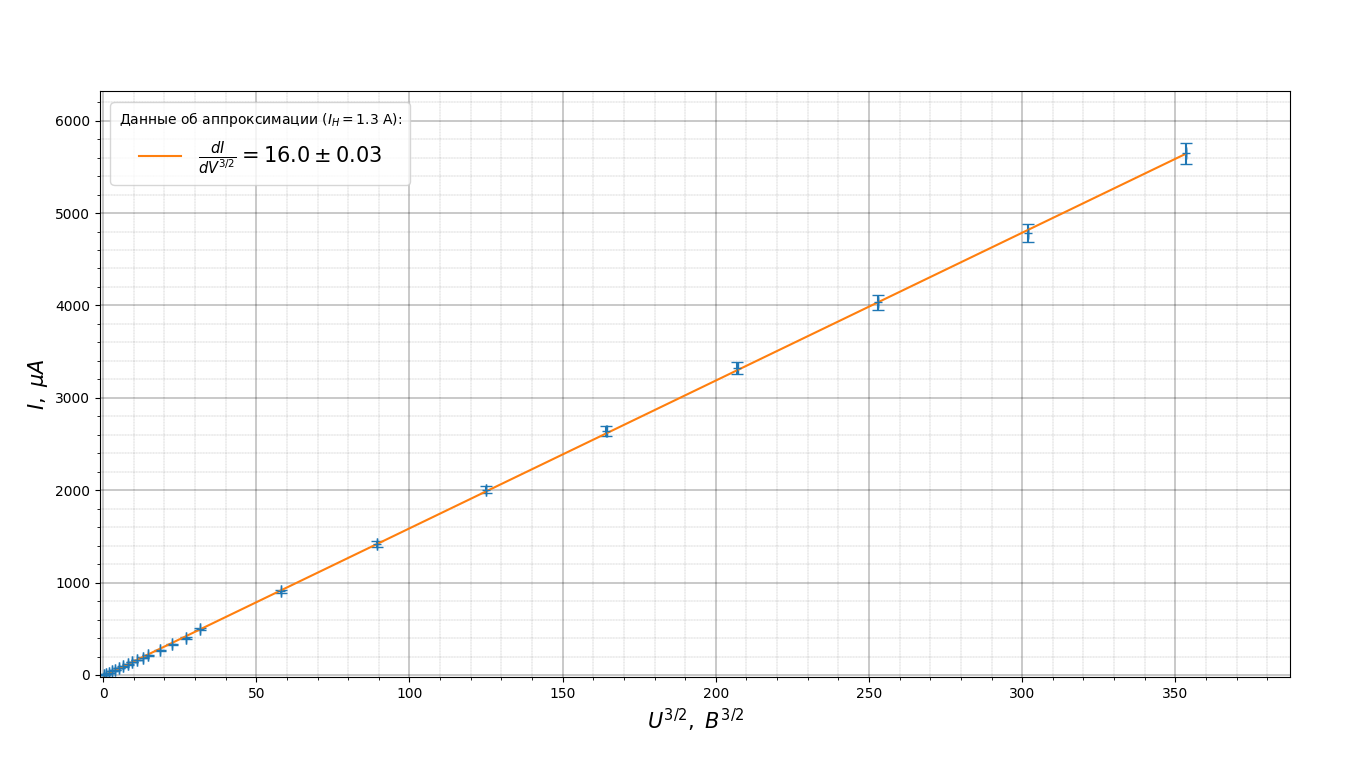
\includegraphics[width=0.9\linewidth]{1.3}
		\caption{Зависимость $I=f(U^{3/2})$, для $I_H = 1.3$ А}
		\label{fig:1}
	\end{figure}
	\begin{figure}[H]
		\centering
		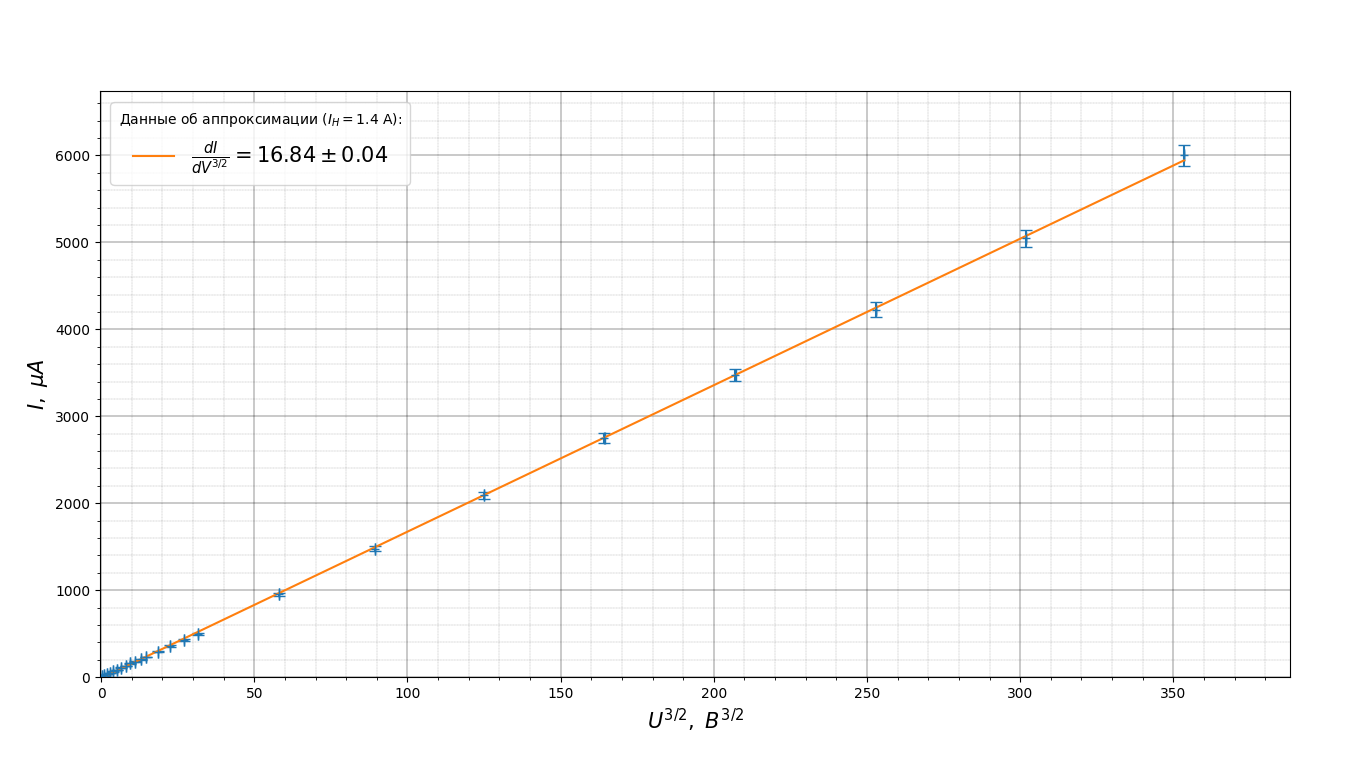
\includegraphics[width=0.9\linewidth]{1.4}
		\caption{Зависимость $I=f(U^{3/2})$, для $I_H = 1.4$ А}
		\label{fig:1}
	\end{figure}
	\begin{figure}[H]
		\centering
		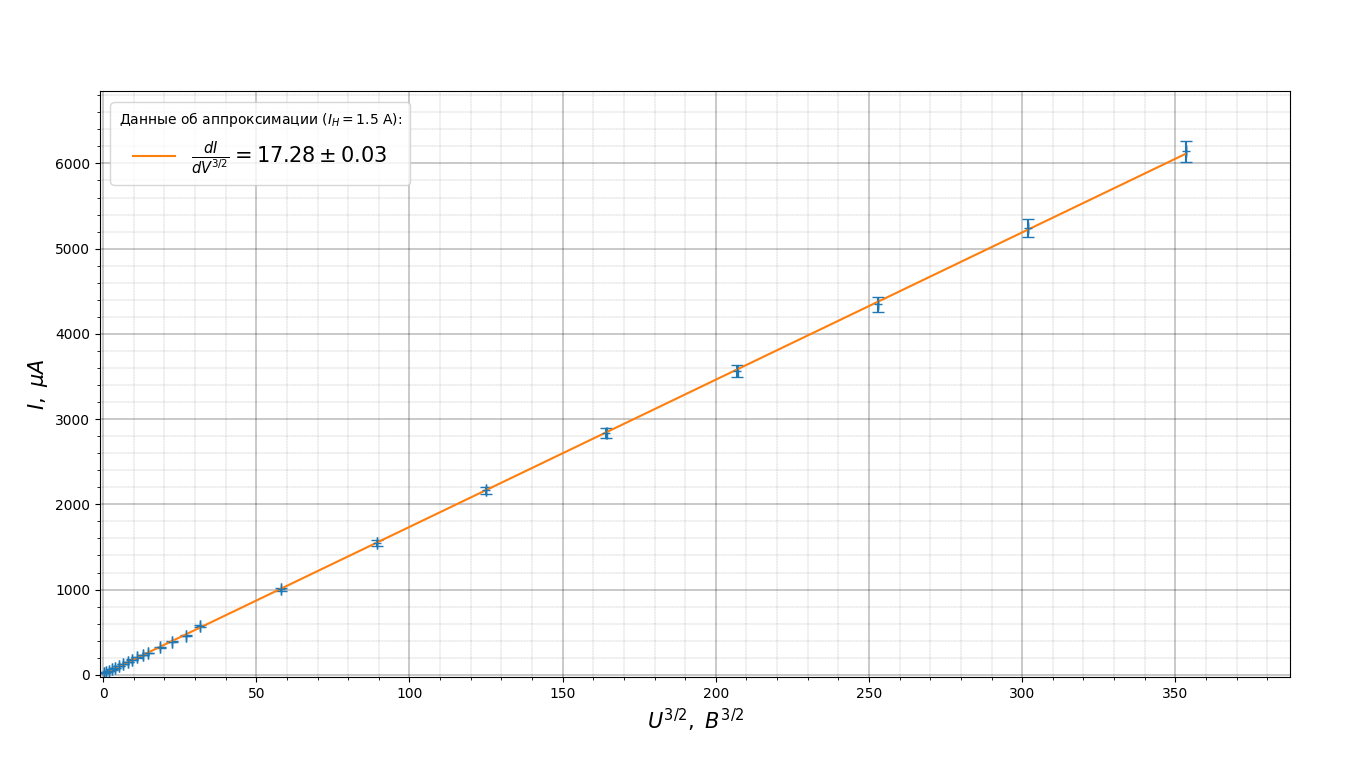
\includegraphics[width=0.9\linewidth]{1.5}
		\caption{Зависимость $I=f(U^{3/2})$, для $I_H = 1.5$ А}
		\label{fig:1}
	\end{figure}
	\begin{figure}[H]
		\centering
		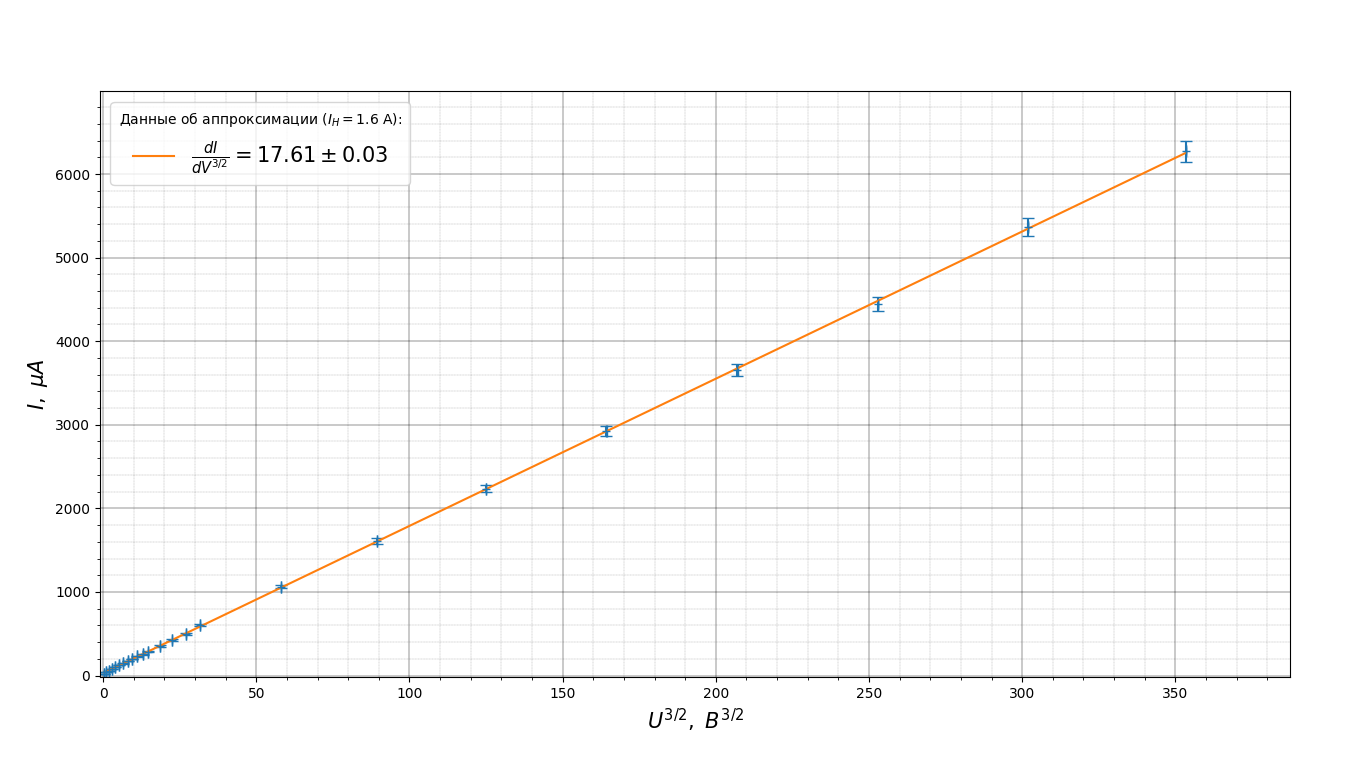
\includegraphics[width=0.9\linewidth]{1.6}
		\caption{Зависимость $I=f(U^{3/2})$, для $I_H = 1.6$ А}
		\label{fig:1}
	\end{figure}
	\subsection{Рассчет удельного заряда электрона}
	В пункте (3.1) получили значение введенного нами коэффициента $k$, а в пункте (3.3) получили значения требуемых производных, отсюда, по формуле (6), вычислим удельный заряд электрона.
	\begin{table}[H]
		\centering
		\begin{tabular}{|c|c|c|c|c|}
			\hline
			\multicolumn{1}{|l|}{$I_H$, А} & \multicolumn{1}{l|}{$\frac{dI}{dV^{3/2}}$} & \multicolumn{1}{l|}{$\sigma(\frac{dI}{dV^{3/2}})$} & \multicolumn{1}{l|}{$\frac{e}{m}, ~\cdot10^{11}$, Кл/кг} & \multicolumn{1}{l|}{$\sigma(\frac{e}{m}), ~\cdot10^{11}$, Кл/кг} \\ \hline
			1.3                       & 16.000                     & 0.028                  & 2.150                  & 0.008                  \\ \hline
			1.4                       & 16.844                     & 0.036                  & 2.383                  & 0.010                  \\ \hline
			1.5                       & 17.279                     & 0.025                  & 2.508                  & 0.007                  \\ \hline
			1.6                       & 17.611                     & 0.026                  & 2.605                  & 0.008                  \\ \hline
		\end{tabular}
		\caption{Зависимость удельного заряда электрона от накального тока}
	\end{table}
	\section{Выводы}
	1) В работе проверили справедливость закона <<трех вторых>>\\
	2) Сняли ВАХ вакуумного диода при различных значениях тока.\\
	3) Рассчитали удельный заряд электрона:\\
	Экспериментально: $\frac{e}{m} = (2.412 \pm 0.008) \cdot 10^{11}$, Кл/кг\\
	Табличное значение: $\frac{e}{m} = 1.76 \cdot 10^{11}$, Кл/кг\\
	Полученное значение сходно по порядку с табличным, однако не попадает в полученную погрешность. Причиною данному могут быть: износ лампы, плохой контакт. Также, видим тенденцию роста при увеличении накального тока, это может быть обусловлено узкой полосой накального тока при котором лампа работает в идеальном режиме (без перегрева и тд.)
\end{document}